\documentclass{beamer}

\usepackage[brazil]{babel}
\usepackage[utf8]{inputenc}
\usepackage{graphicx}

\usetheme{Warsaw}
\usecolortheme{beetle}

\begin{document}

	\title{Robô Explorador de Ambientes}
	\author{Luis Camargo \newline \  Marcelo Teider \newline \  Matheus Araujo}
	\institute{Universidade Tecnológica Federal do Paraná}

	\date{7 Dez 2011}

	\frame{\titlepage}

	\frame{
		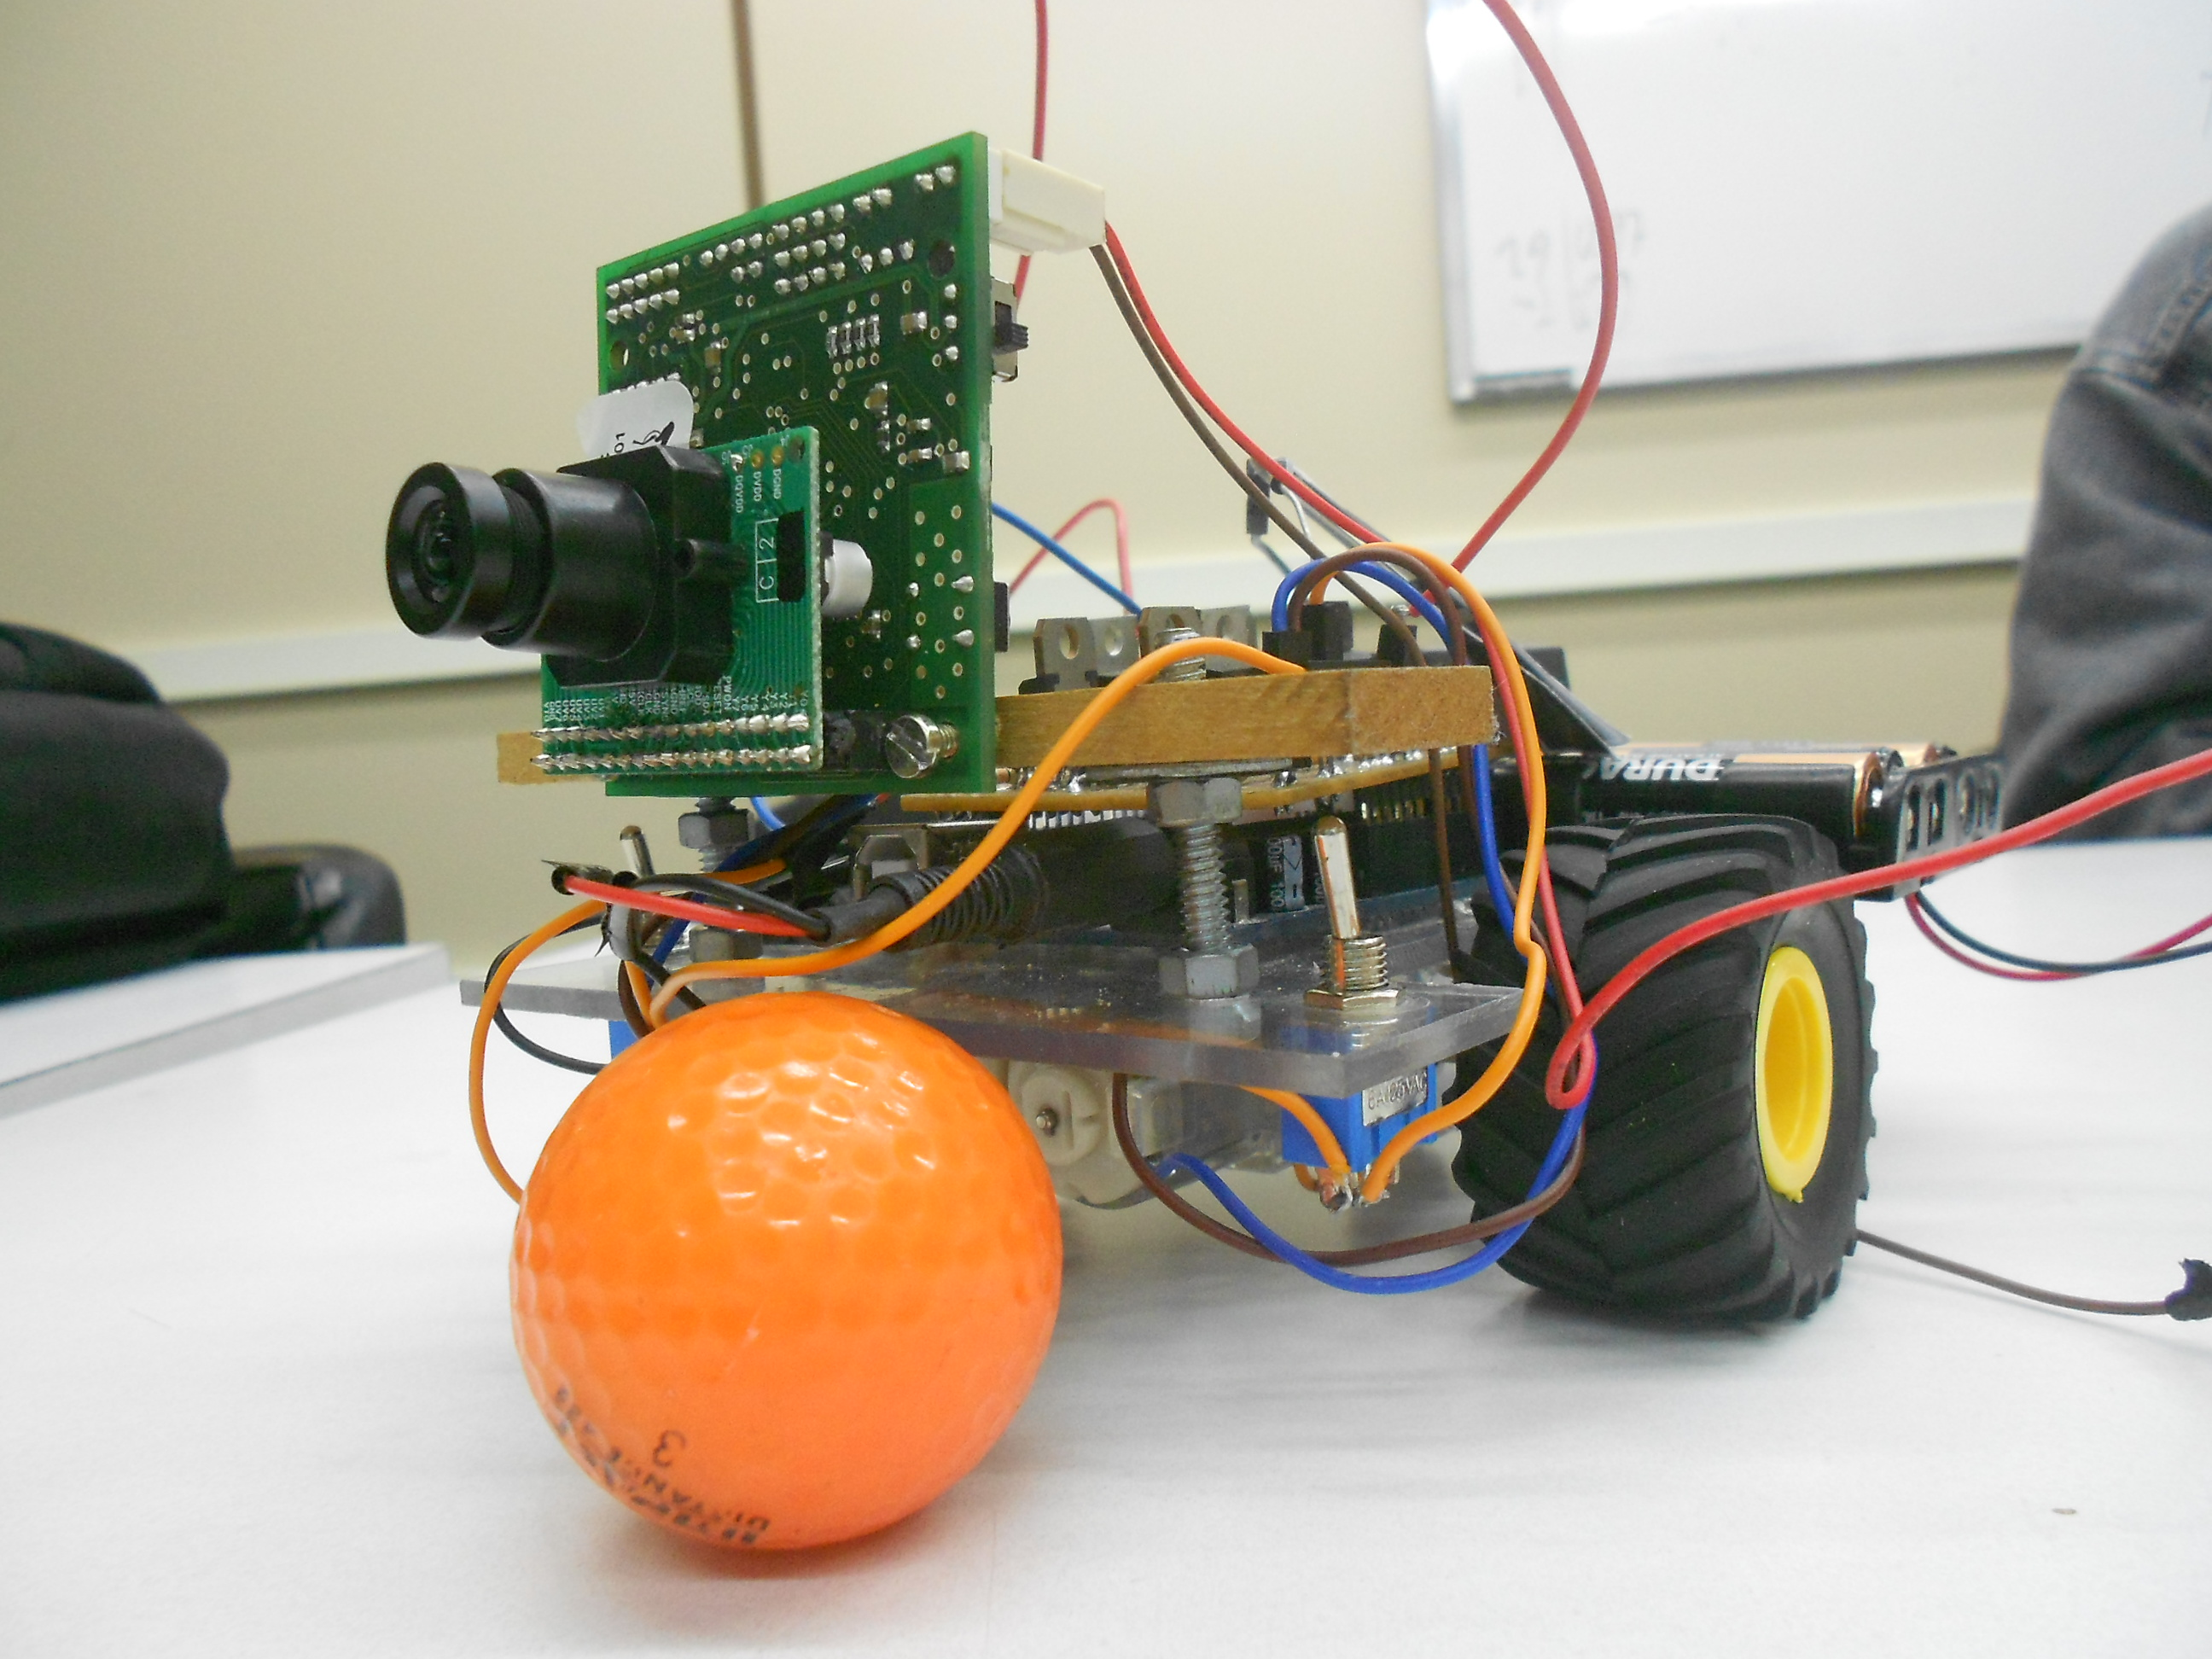
\includegraphics[width=11cm,height=7cm]{images/robo}
	}

	\section{Introdução}
	
	\frame{

		\frametitle{Introdução}
		
		\begin{itemize}
			
			\item<1-> \textbf{O que é?}

				\begin{itemize}

					\item<2-> Projeto de um robô que explora ambientes em busca de um objeto específico usando uma câmera e uma bússola como sensores.

				\end{itemize}

			\item<3-> \textbf{Por quê?}

				\begin{itemize}

					\item<4-> Porque é legal!

					\item<5-> Robôs exploradores têm diversas aplicações, desde atividades em hospitais a explorações espaciais.

				\end{itemize}
			
		\end{itemize}

	}

	\frame{

		\frametitle{Visão Geral}

		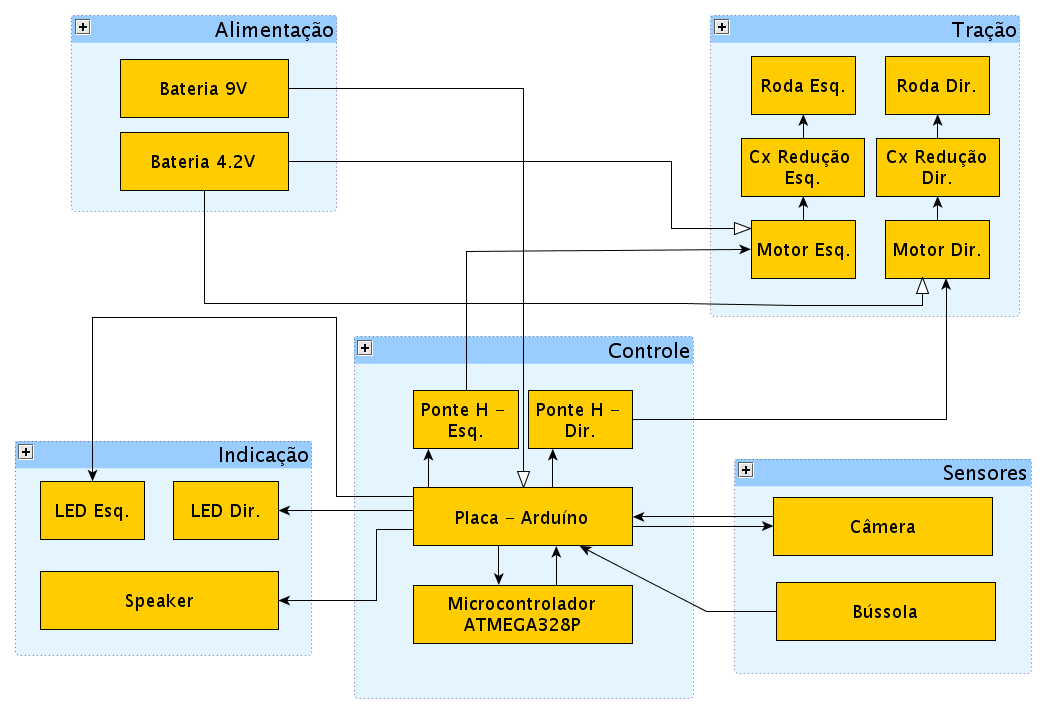
\includegraphics[width=11cm, height=7cm]{images/robo_geral}

	}	

	\section{Projeto Mecânico}

		\frame{

			\frametitle{Projeto Mecânico}

			\begin{itemize}

				\item<1-> Robô reutilizado do projeto \textbf{Robô Explorador de Labirintos 2D}, Bruno Meneguele, Fernando Padilha e Vinicius Arcanjo, apresentado a esta disciplina no primeiro semestre de 2011.

				\item<2-> Foram reaproveitados: chassi, motor, caixa de redução, rodas, \textit{Arduíno}. 

				\item<3-> Os sensores de luz infravermelha foram substituídos pela câmera.

			\end{itemize}

		}


		\subsection{Robô}

			\frame{

				\frametitle{Robô}


				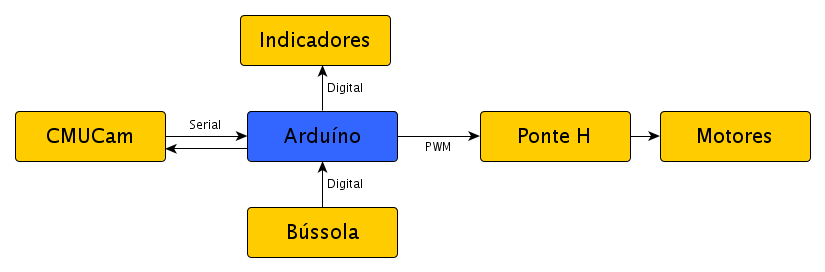
\includegraphics[width=7cm, heigh=4cm]{images/processo_arduino}


				\begin{itemize}


					\item<1->O projeto do robô está centrado no \textit{Arduíno}.

					\item<2->Ele é o responsável por receber as decisões tomadas pela câmera e atuar sobre os sistemas do robô.

				\end{itemize}

			}

		\subsection{Comunicação}

			\frame{

				\frametitle{Comunicação}

			}


	\section{Sensores}

		\subsection{Sistema de Visão}
	
		\frame{

			\frametitle{Sistema de Visão}
		
		}

		\frame{
			
			\frametitle{\textit{Track-color}}

			\begin{itemize}

				\item Algoritmo que, a partir de uma faixa RGB definida, retorna da imagem as coordenadas de um retângulo com o centróide e a densidade de \textit{pixels} daquela cor.

			\end{itemize}

		}

		\frame{

			\frametitle{\textit{Track-color}}

			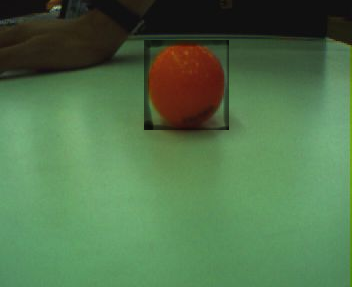
\includegraphics[width=5.5cm, height=3.5cm]{images/cam01.png}

			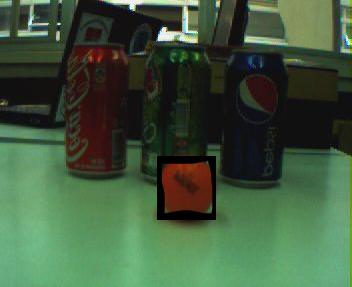
\includegraphics[width=5.5cm, height=3.5cm]{images/cam02.png}

		}

		\subsection{Bússola}

		\frame{

			\frametitle{Bússola}

		}

	\section{Exploração}
	
		\frame{
		
			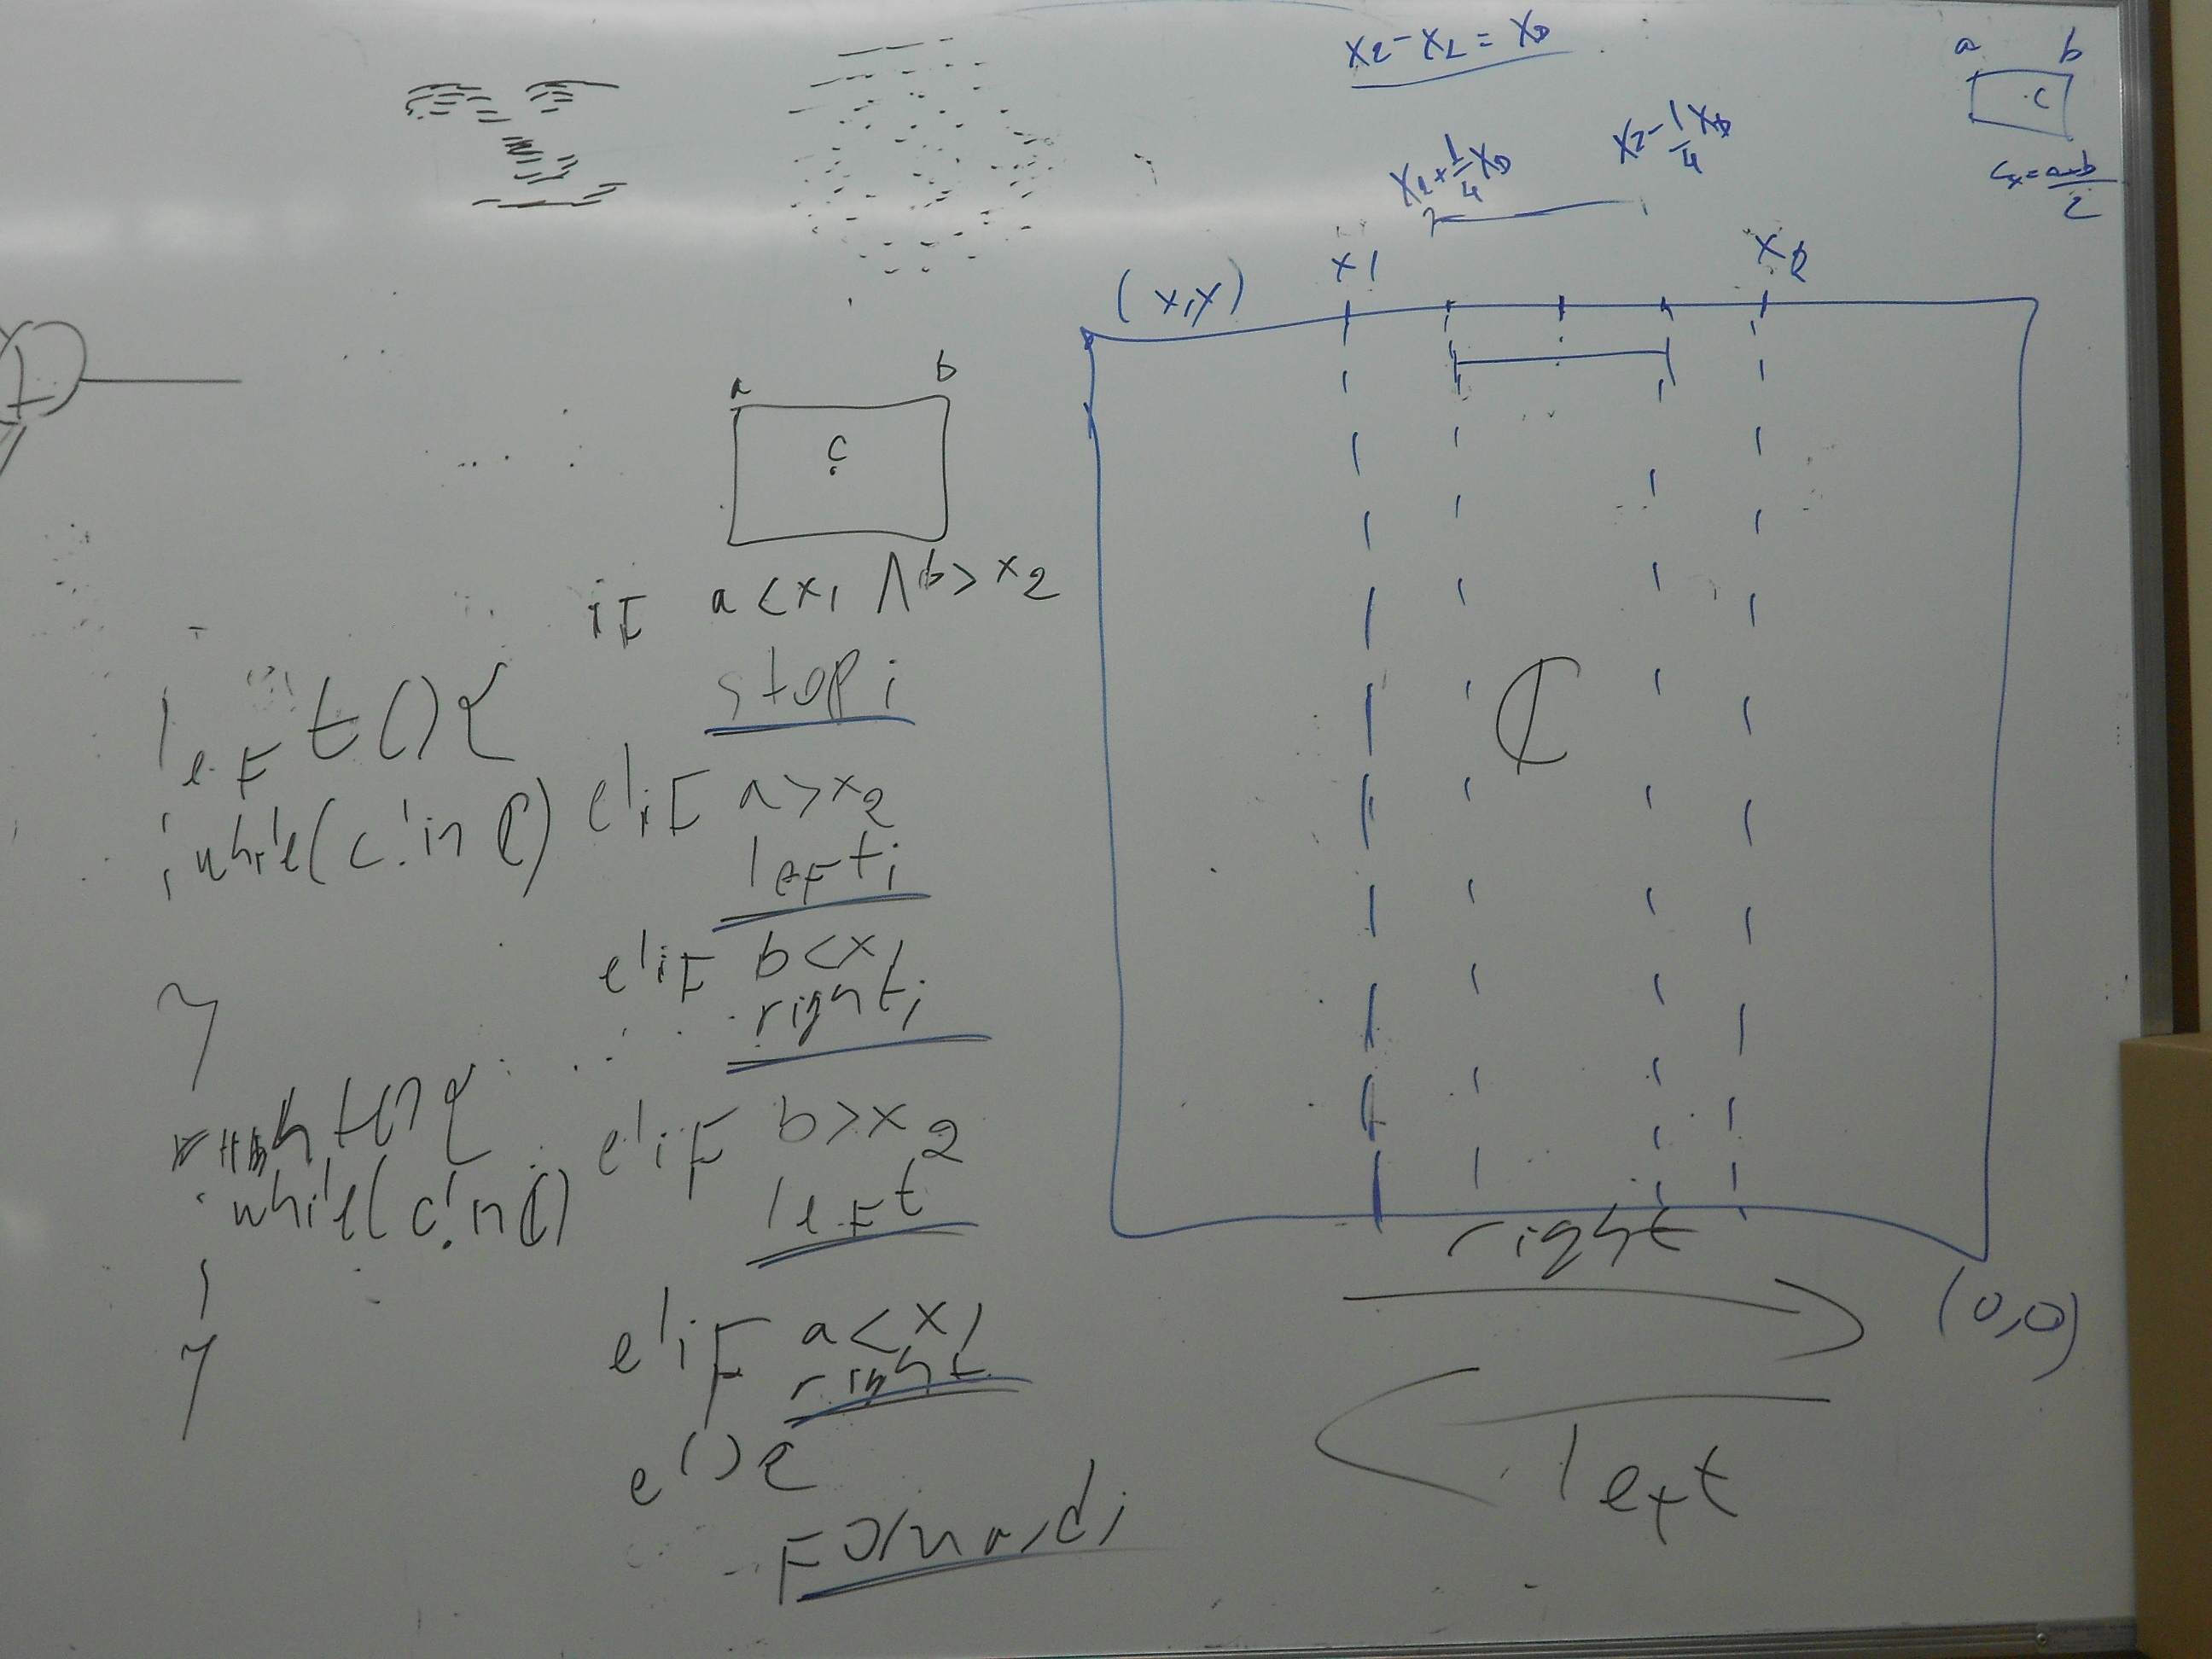
\includegraphics[width=11cm, height=7cm]{images/algoritmo_navegacao}
			
		}

		\frame{

			\frametitle{Exploração}

		}

	\section{}

		\frame{
		
			\frametitle{Agradecimentos}

			\begin{itemize}

				\item Professores Myriam Delgado, Hugo Vieira, Mário Sérgio de Freitas, Cesar Tacla, João Fabro

				\item Colegas Bruno Meneguele, Fernando Padilha, Vinicius Arcanjo

				\item Colegas Claudio Akio, Kaya Sumire Abe, Lucas Paiva

				\item Marceneiros do Almoxarifado da UTFPR

			\end{itemize}
		
		}





\end{document}
